\documentclass[11pt]{article}
\renewcommand{\rmdefault}{ptm}
\usepackage[scaled=0.92]{helvet}
\usepackage{courier,xcolor,colortbl,listings,parskip,graphicx,fancyvrb,fancyhdr,lastpage}
\usepackage{float,framed}
\normalfont
\usepackage[T1]{fontenc}
%\setlength{\parskip}{7pt}
\usepackage[toc,page]{appendix}
\usepackage[hmargin=2.5cm,vmargin=2cm]{geometry}
\usepackage[utf8]{inputenc}
\usepackage[brazil]{babel}
\usepackage{fancyvrb}
\pagestyle{fancy}
\setlength{\headheight}{120pt}
\setlength{\headsep}{30pt}
\setlength{\textheight}{550pt}
\renewcommand{\headrulewidth}{0pt}
\lhead{}
\rhead{}
\chead{
\includegraphics{brasao.jpg}\\
        \large \textbf{PRESIDÊNCIA DA REPÚBLICA}\\
        \large SECRETARIA-GERAL\\
        \large Secretaria-Executiva}
\cfoot{}
\rfoot{\thepage /\pageref{LastPage}}
\hyphenation{par-ti-ci-pa-ção}

\newcommand{\MyName}{Joenio Marques da Costa}
\newcommand{\MyEmail}{joenio@colivre.coop.br}
\newcommand{\ContractNumber}{2013/000564}
\newcommand{\ProjectCode}{Projeto PNUD BRA/12/018}
\newcommand{\NomeSecretaria}{Secretaria Geral da Presidência da República}
\newcommand{\SiglaSecretaria}{SG/PR}
\newcommand{\ProductNumber}{02}
\newcommand{\ProductDescription}{"Documento com análise de arquiteturas de
        sistemas de identidade distribuída, estratégia de implantação
        considerando os sites parceiros e contendo propostas de códigos."
}
\newcommand{\MesEntrega}{Abril de 2014}
\newcommand{\DiaEntrega}{21}
\bibliographystyle{ieeetr}{}

\begin{document}
\lstset{language=Ruby}
\definecolor{light-gray}{gray}{0.95}
\lstdefinestyle{codeFrame}{backgroundcolor=\color{light-gray},frame=lines}

\textbf{\ProjectCode \ -} \ProductDescription

\vspace{3cm}

\begin{minipage}{0.5\textwidth}
  \textbf{Consultora: \MyName}
  \newline
  \textbf{Contrato nº: \ContractNumber}
  \newline
  \textbf{Produto / nº: \ProductNumber}
\end{minipage}

\vspace{2cm}

\textbf{Assinatura do Consultor}

\begin{framed}
Local e data: Brasília/DF, \line(1,0){20} \ de \line(1,0){100} \ de 2014
\newline
\newline
Assinatura do Consultor: \line(1,0){300}
\end{framed}

\vspace{1cm}

\textbf{Assinatura do Supervisor}

\begin{framed}
Atesto que os serviços foram prestados conforme estabelecido no Contrato
de Consultoria.
\newline
\newline
Local e data: Brasília/DF, \line(1,0){20} \ de \line(1,0){100} \ de 2014
\newline
\newline
Assinatura e Carimbo: \line(1,0){300}
\end{framed}

\clearpage
\newcolumntype{g}{>{\columncolor{light-gray}}l}

\begin{center}
  \begin{tabular}{| g | p{10cm} |}
    \hline
    \textbf{Título} & \ProductDescription \\ \hline
    \textbf{Língua do documento} & Português - Brasil \\ \hline
    \textbf{Documentação de referência} & Português \\ \hline
    \textbf{Unidade responsável} & \NomeSecretaria \
(\SiglaSecretaria) \\ \hline
    \textbf{Criador} & \MyName - \MyEmail \\ \hline
    \textbf{Taxonomias} & Desenvolvimento \\ \hline
    \textbf{Data de aprovação} & mês de ano \\ \hline
    \textbf{Público} & \SiglaSecretaria, Parceiros e Sociedade
Civil \\ \hline
    \textbf{Aplicabilidade} & Explicar isso aqui \\ \hline
    \textbf{Faz parte do} & \ProjectCode \\ \hline
    \textbf{Em conformidade com a} & \NomeSecretaria \\ \hline
    \textbf{Documentos anexos} & Nenhum \\ \hline
    \textbf{Revisado em} & dia mês ano \\ \hline
  \end{tabular}
\end{center}

\clearpage

\tableofcontents
\clearpage
\listoffigures

\clearpage

\section{Apresentação}

Em consonância com os objetivos e cronograma previsto no âmbito do
projeto BRA/12/018:
\textbf{Desenvolvimento de Metodologias de Articulação e Gestão de
Políticas Públicas para Promoção da Democracia Participativa},
firmado entre a Secretaria-Geral da Presidência da República
(SG/PR) e o Programa das Nações Unidas para o Desenvolvimento (PNUD),
o presente documento apresenta \ProductDescription.

Essa proposta está configurada como produto \ProductNumber~da consultoria técnica
para especificação da construção dos códigos das metodologias de
organização da informação e interação participativa do portal de
participação social.


\section{SSO - Single Sign-on}

\subsection{O que é SSO?}

Single Sign-on, ou Web Browser Single Sign-on é a propriedade de controle de
acesso a sistemas Web onde usuários efetuam login apenas uma vez e ganham acesso a
outros sistemas que tenham relação com tal sistema sem a necessidade de fornecer
suas credenciais de autenticação uma segunda vez. Os sistemas que possuem
relação são definidos previamente pela implementação e configuração do
ambiente de SSO e é feito pelos desenvolvedores e administradores dos sistemas envolvidos.
Analogamente, single sign-off é a propriedade inversa, onde o usuário finaliza
sua sessão de login em um sistema e de forma automática ele é deslogado também
dos outros sistemas que façam parte deste mesmo ambiente.

Usualmente, ambientes SSO compartilham servidores de autenticação para servir
cada aplicação, com objetivo de autenticar e garantir que usuários não
necessitem entrar com suas credenciais de autenticação mais de uma
vez\cite{wikipediaSingleSignOn}. Estes servidores
fornecem serviços de autenticação em rede para aplicações externas, a
autenticação pode ser feita por diversos métodos, mas normalmente usa-se
usuário/senha\cite{wikipediaAuthenticationServer} em
aplicações Web.

O uso de SSO aumenta drasticamente o impacto negativo em caso de roubo de
informações, uma vez que o acesso a esta informação possibilita acesso a
diversos sistemas, portanto a proteção dessas informações devem ser redobradas.
É preciso também ter cuidado com a disponibilidade do serviço, uma vez
que sua queda implica em indisponibilidade dos serviços que fazem parte do
ambiente de SSO.

\subsection{SSO no Noosfero}

O Noosfero não implementa mecanismos de SSO, nem há referências na comunidade
de utilização dele num ambiente como este. O mecanismo de autenticação presente
no Noosfero está implementado nos seguintes arquivos:

\begin{itemize}
  \item noosfero/lib/authenticated\_system.rb
  \item noosfero/app/controllers/public/account\_controller.rb
  \item noosfero/app/model/user.rb
\end{itemize}

Esta implementação presente no {\it core} do Noosfero realiza autenticação
através de usuário/senha e armazena estas informações em banco de dados de
forma encriptada. É possível alterar o método de autenticação através de
plugins, um exemplo é o plugin Ldap distribuído junto ao Noosfero em:

\begin{itemize}
  \item noosfero/plugins/ldap
\end{itemize}

Este plugin possibilita realizar autenticação a partir de um servidor LDAP.

\subsection{Qual problema SSO resolve?}

SSO resolve um problema bem comum e conhecido, o usuário de um serviço Web
(site, sistema, rede social, etc) quer logar apenas uma vez e manter sua
sessão entre diversos serviços (outros sites, outras redes, etc) sem
necessidade de fornecer seus dados de acesso uma segunda vez.

A solução para esta questão precisa lidar com uma política segurança e
privacidade implementada nos Navegadores Web, esta política, chamada Same
Origin Policy\cite{wikipediaSameOriginPolicy} é
uma recomendação do W3C e previne que documentos em diferentes domínios afetem
e compartilhem dados com outros domínios, isso previne, por exemplo, ataques de
cross-site scripting.

Inúmeras soluções foram propostas para contornar esta política, JSONP, CORS,
easyXDM, entre outras\cite{stackoverflowAjax}, todas elas se tornaram
obsoletas após a recomendação do W3C chamada "Web
Messaging"\cite{w3cWebmessaging}, uma técnica que permite documentos em
diferentes domínios compartilhar dados. A maioria dos Navegadores Web atuais
implementam Web Messaging\cite{wikipediaWebmessaging}
\cite{stackexchangeJSONP} \cite{webMessagingOpenBlog}.

\subsection{Como SSO funciona?}

Existem muitas formas de implementar SSO: Kerberos, Smart card, CAS, OTP,
entre outras, cada uma com sua própria
estratégia\cite{opengroupSSO}. A solução
SiteMinder\cite{siteminderCA}
da "CA Technologies", por exemplo, implementa SSO da seguinte
forma\cite{siteminderDOCS}:

\begin{itemize}
  \item{Usuário autentica uma vez}
  \item{O navegador faz cache da autenticação e seta um cookie com
        informações de single sign-on}
  \item{O cookie fornece informações de sessão, assim o usuário pode acessar
        outros sites sem necessidade de re-autenticar}
\end{itemize}

A Figura~\ref{fig:sso-siteminder} traz um diagrama exemplificando esta
solução. A solução SiteMinder é um sistema centralizado de gerenciamento de
acesso Web da empresa "CA Technologies", que implementa uma série de soluções,
além de SSO.

\begin{figure}[h]
\center
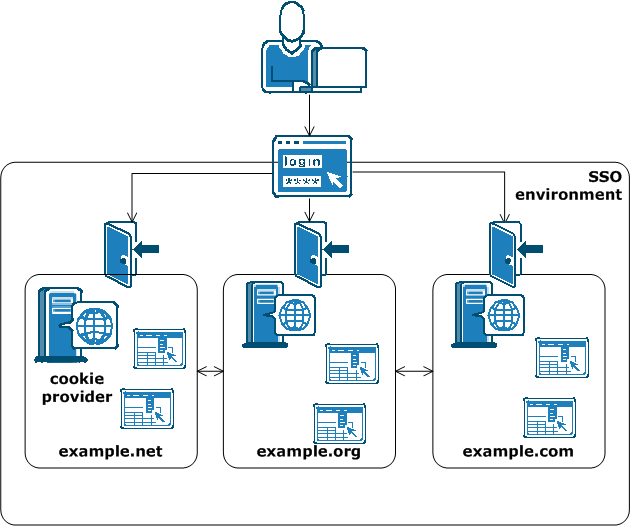
\includegraphics[scale=0.6]{sso-siteminder.png}
\caption{Exemplo de implementação de SSO do SiteMinder}
\label{fig:sso-siteminder}
\end{figure}

\subsection{Quais soluções de SSO existem?}

A seguir é apresentada uma lista de soluções em software livre para SSO
elaborada com base no artigo da Wikipedia em:

\begin{itemize}
  \item http://en.wikipedia.org/wiki/List\_of\_single\_sign-on\_implementations
\end{itemize}

\subsubsection{Accounts \& SSO}

Framework contendo um conjunto de componentes e bibliotecas para autenticação
de contas de usuários online para clientes Desktops, sistemas Linux e POSIX.

Mais em:
\begin{itemize}
  \item{http://en.wikipedia.org/wiki/Accounts\_\&\_SSO}
\end{itemize}

{\bf Avaliação:} {\it Não é uma opção válida para ser implantado no portal de
participação social Participa.br pois é voltado para clientes desktop.}

\subsubsection{Central Authentication Service (CAS)}

Protocolo de Single Sign-on para a Web. O nome CAS refere-se também a uma
implementação deste mesmo protocolo. O fluxo durante a autenticação é o
seguinte:

\begin{itemize}
  \item{Cliente visita uma aplicação que requisita autenticação}
  \item{A aplicação redireciona o Cliente para o CAS}
  \item{CAS valida atenticidade do Cliente (geralmente contra um banco, Kerberos, Active Directory, etc)}
  \item{Se a autenticação tem sucesso, o CAS retorna o cliente para a aplicação, passando um ticket de segurança}
  \item{A aplicação valida o ticket contactando o CAS}
  \item{O CAS dá a informação com segurança à aplicação que o usuário foi autenticado com sucesso}
\end{itemize}

A implementação oficial do CAS é em Java e é mantido, hoje, pelo grupo
JASIG\cite{jasigSite}, existem implementações oficiais de cliente em várias
linguagens, como: .NET, PHP, Perl, Apache, etc.  A partir da versão 3.5
adicionou suporte a OAuth\cite{oauthJasig}, tanto cliente quanto servidor.

\begin{figure}[h]
\center
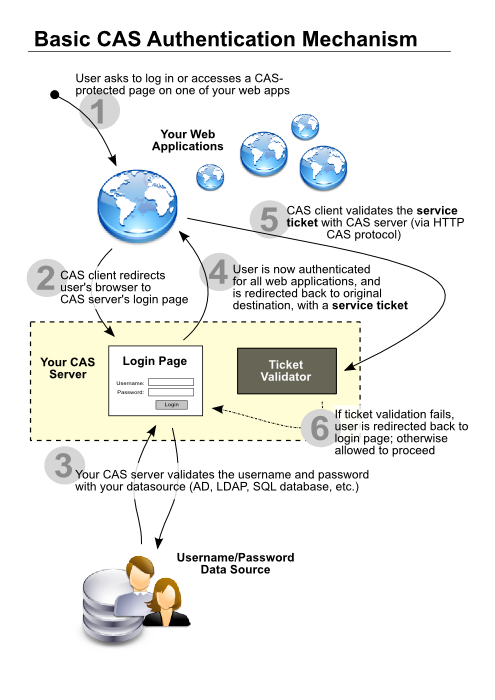
\includegraphics[scale=0.4]{sso-rubycas.png}
\caption{Diagrama do RubyCAS, implementação do protocolo CAS em Ruby}
\label{fig:sso-rubycas}
\end{figure}

O artigo {\it Approaches and challenges for a single sign-on enabled extranet
using Jasig CAS}\cite{approachesAndChallengesSSO} descreve a experiência em
configurar single sign-on em um ambiente de intranet usando o CAS e outros
software livres, e faz uma boa avaliação das tecnologias envolvidas, como
OpenID, OAuth, etc.

CAS centraliza a autenticação e é recomendável de ser utilizado quando todas
as aplicações autenticam numa mesma base de credenciais de autenticação. É
geralmente a melhor escolha para grandes organizações, onde se quer
centralizar a base de usuários, como universidades por exemplo.

Mais em:
\begin{itemize}
  \item{http://en.wikipedia.org/wiki/Central\_Authentication\_Service}
  \item{http://www.jasig.org/cas/protocol}
\end{itemize}

{\bf Avaliação:} {\it Implementação madura contendo um bom conjunto de
técnicas para implementação de SSO, incluindo suporte a OAuth, OpenID, SAML, LDAP,
etc. É uma opção recomendada.}

\subsubsection{Distributed Access Control System (DACS)}

DACS é um sistema de SSO leve combinado com mecanismos de autenticação e
controle de acesso para Web escrito em C/C++. Possui suporte para integrar com
diversos mecanismos de autenticação, como X.509, PAM, LDAP, etc. Possui módulo
de autenticação para servidor Web Apache\cite{webServicesRoleBased}.

O Debian utiliza DACS para prover SSO entre alguns dos seus servidores de
desenvolvimento do projeto.

Mais em:
\begin{itemize}
  \item{http://en.wikipedia.org/wiki/Distributed\_Access\_Control\_System\_(DACS)}
  \item{https://wiki.debian.org/DebianSingleSignOn}
\end{itemize}

{\bf Avaliação:} {\it Recomendado.}

\subsubsection{Enterprise Sign On Engine}

Plataforma de SSO, controle de acesso e federação compatível com SAML 2.0
e parcialmente compatível com
XACML\cite{wikipediaXACML}.

Desenvolvido em Java, possui suporte a Tomcat, Apache e IIS.

Mais em:
\begin{itemize}
  \item{http://en.wikipedia.org/wiki/Enterprise\_Sign\_On\_Engine}
\end{itemize}

{\bf Avaliação:} {\it Nenhuma referência encontrada sobre seu uso em produção,
não recomendado para o portal de participação social Participa.br.}

\subsubsection{FreeIPA}

Solução da RedHat para SSO e "Policy and Audit". É comparável a solução
"Novell's Identity Manager" ou "Microsoft's Active Directory" pois tem
objetivos e mecanismos similares.

Usa as soluções 389 Directory Server, MIT Kerberos 5, Apache HTTP e Python. A
partir da versão 3.0.0 adicionou suporte a Samba para integração com Microsoft
Active Directory.

Mais em:
\begin{itemize}
  \item{http://en.wikipedia.org/wiki/FreeIPA}
\end{itemize}

{\bf Avaliação:} {\it Esta solução é incialmente voltada para ambientes de
rede desktop e não atende aos requisitos do Participa.br.}

\subsubsection{IBM Enterprise Identity Mapping}

Framework para mapear identidades de usuários em várias plataformas distintas,
pouca informação disponível na Web.

Mais em:
\begin{itemize}
  \item{http://en.wikipedia.org/wiki/IBM\_Enterprise\_Identity\_Mapping}
\end{itemize}

{\bf Avaliação:} {\it Voltado apenas para integrar soluçoes da própria
IBM.}

\subsubsection{JBoss SSO}

Faz parte da suíte de soluções JBoss SOA, permite single sign-on, sign-off e
acesso federado a múltiplas aplicações e recursos computacionais em rede.

Dentre várias funcionalidades o JBoss SSO inclue:

\begin{itemize}
  \item{Integração entre aplicações e módulos baseados no padrão SAML}
  \item{Abordagem descentralizada}
  \item{Habilidade de conectar a diferentes sistemas de armazenamento}
\end{itemize}

Mais em:
\begin{itemize}
  \item{http://en.wikipedia.org/wiki/JBoss\_SSO}
\end{itemize}

{\bf Avaliação:} {\it Solução madura, possível alternativa a ser utilizada.}

\subsubsection{JOSSO}

Java Open Single Sign On (JOSSO) é uma solução de SSO para aplicações Web.
Baseado em Java EE, permite mútiplos servidores web autenticar
usuários através de suas credenciais. JOSSO se comunica com o armazenamento das
credenciais por LDAP ou JDBC e fornece interface via SOAP sob o protocolo HTTP
para permitir fácil integração com aplicações não-Java.

Mais em:
\begin{itemize}
  \item{http://en.wikipedia.org/wiki/JOSSO}
\end{itemize}

{\bf Avaliação:} {\it Solução madura, possível alternativa a ser utilizada.}

\subsubsection{Kerberos}

Protocolo de autenticação em rede baseado em 'tickets', permite comunicação
entre nós sob uma rede não-segura de forma segura. Foi projetado
principalmente com um modelo cliente-servidor, isso provê autenticação tanto
de usuários quanto de servidores. Veja na Figura~\ref{fig:kerberos} um exemplo
de negociação com o Kerberos.

\begin{figure}[h]
\center
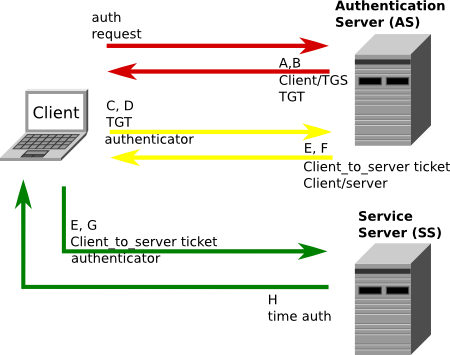
\includegraphics[scale=0.6]{kerberos.png}
\caption{Diagrama de negociação do Kerberos}
\label{fig:kerberos}
\end{figure}

Mais em:
\begin{itemize}
  \item{http://en.wikipedia.org/wiki/Kerberos\_(protocol)}
\end{itemize}

{\bf Avaliação:} {\it Protocolo de autenticação, não é uma solução para SSO.}

\subsubsection{OpenAM}

Provê single sign-on de forma transparente em infraestrutura de redes. Escrito
em Java, suporte a mais de 20 tipos de autenticação, possui suporte a SAML e
implementa sistema de autorização baseado em XACML. Veja um exemplo na
Figura~\ref{fig:opensso} de uso do OpenAM em um portal de viagens.

\begin{figure}[h]
\center
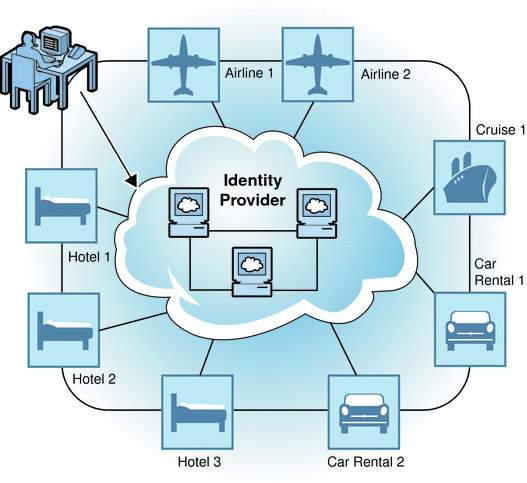
\includegraphics[scale=0.5]{opensso.png}
\caption{Exemplo de federação com OpenAM para um portal de viagens}
\label{fig:opensso}
\end{figure}

O OpenSSO, projeto que deu origem ao OpenAM, foi utilizado pela CPqD para
implantar Single Sign-on entre diversas aplicações e é um bom caso de uso
desta plataforma em um ambiente real, mais detalhes no link abaixo:

\begin{itemize}
  \item{https://blogs.oracle.com/superpat/entry/opensso\_at\_cpqd}
\end{itemize}

Mais em:
\begin{itemize}
  \item{http://en.wikipedia.org/wiki/OpenAM}
\end{itemize}

{\bf Avaliação:} {\it Possível alternativa de ser utilizada, madura, bem
documentada e bastante utilizada, suporta: OAuth, SAML, Kerberos, LDAP, etc.}

\subsubsection{Pubcookie}

Protocolo (e software) de SSO, o processo de autenticação se dá da seguinte
forma:

\begin{itemize}
  \item{Quando usuário acessa a aplicação, Pubcookie seta 2 cookies, pré-sessão e concessão de requisição}
  \item{Redireciona usuário para página de login}
  \item{Usuário fornece login e senha, se o login for com sucesso, seta 2 cookies, login e concessão}
\end{itemize}

Mais em:
\begin{itemize}
  \item{http://en.wikipedia.org/wiki/Pubcookie}
\end{itemize}

{\bf Avaliação:} {\it O último release do projeto é de 2010, não recomendado
como possível solução de SSO para o portal Participa.br}

\subsubsection{SAML}

Linguagem de marcação para definir comunicação sobre autenticação e autorização

Security Assertion Markup Language (SAML) é uma linguagem de marcação baseada
em XML para troca de dados de autenticação e autorização definido pelo OASIS
Security Services Technical Committee. O SAML é principalmente desenvolvido
para ser aplicado em Web Browser Single Sign-on.

A especificação SAML define 3 papéis:
\begin{itemize}
  \item{Principal (geralmente um usuário)}
  \item{Provedor de identidade (IdP)}
  \item{Provedor de serviço (SP)}
\end{itemize}

A interação entre eles está representada na Figura~\ref{fig:saml2}.

\begin{figure}[h]
\center
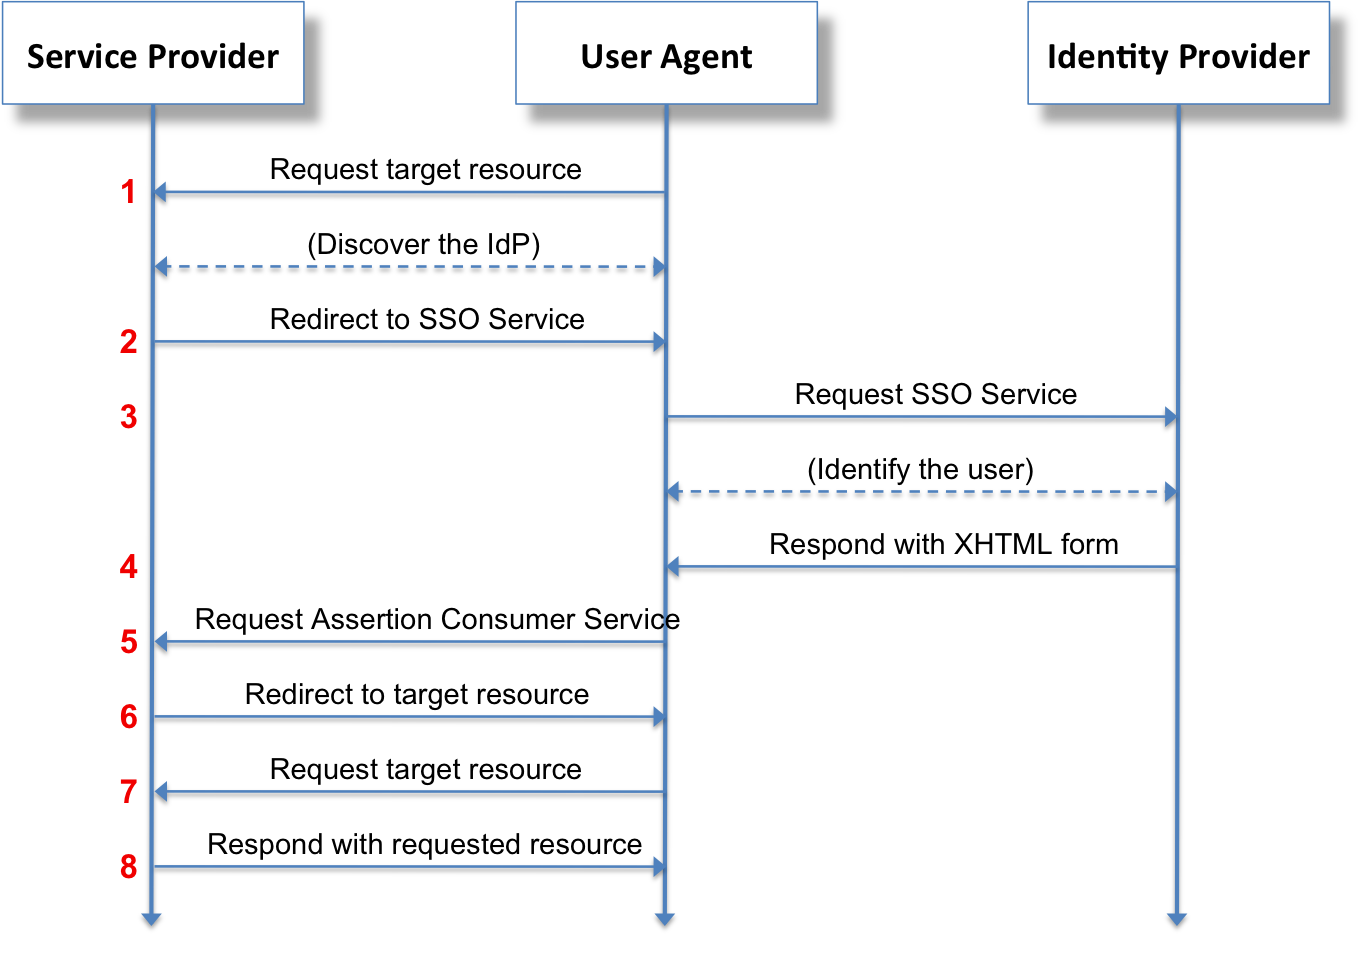
\includegraphics[scale=0.5]{saml2.png}
\caption{Single Sign-on com SAML2}
\label{fig:saml2}
\end{figure}

Mais em:
\begin{itemize}
  \item{http://en.wikipedia.org/wiki/Security\_Assertion\_Markup\_Language}
\end{itemize}

{\bf Avaliação:} {\it Não uma solução de SSO em sí, é suportado por várias
soluções, é altamente recomendado que a solução adotada no Participa.br
suporte este padrão.}

\subsubsection{Shibboleth}

Middleware para SSO e autenticação baseado em SAML.

Mais em:
\begin{itemize}
  \item{http://en.wikipedia.org/wiki/Shibboleth\_(Internet2)}
\end{itemize}

{\bf Avaliação:} {\it É uma possível alternativa a ser utilizada no
Participa.br, tem boas referências de uso na prática como por exemplo a
iniciativa das universidades do Reuino Unido chamada OpenAthens.}

\subsubsection{ZXID}

Kit de gerenciamento de identidade SAML 2.0. Compatícel co SAML 2.0, Liberty
ID-WSF 2.0 e XACML 2.0. Implementado em C com, possui poucas dependencias
externas, fornece bibliotecas para PHP, Perl e Java via SWIG.

Mais em:
\begin{itemize}
  \item{http://en.wikipedia.org/wiki/ZXID}
\end{itemize}

{\bf Avaliação:} {\it Não recomendado.}

\section{IdP - Identity Provider}

\subsection{O que é IdP?}

Identity Provider, ou Provedor de Identidade, é o serviço responsável por
gerenciar informações de identidade entre sistemas, usuários ou outros atores,
provendo através de um módulo interno ou externo serviço de autenticação e
autorização, de forma segura, afim de verificar a autenticidade.

Um provedor de identidade fornece uma alternativa para que vários serviços web
distintos autentiquem seus usuários através dele, de forma que um usuário pode
ter apenas um login/senha e autenticar em vários serviços com este mesmo
login/senha. Isto não implica em Single Sign-on, pois com um provedor de
identidade apenas o usuário ainda precisa passar por uma etapa de
autenticação, num ambiente de SSO isto fica transparente e o usuário ao logar
num sistema Web não precisa passar pela etapa de autenticação ao acessar um
segundo serviço.

Uma solução de SSO é composta usualmente de ao menos 3 componentes:

\begin{itemize}
  \item{Usuário/cliente, geralmente usa-se os termo {\it Principal}}
  \item{Provedor de identidade, {\it IdP - Identity Provider}}
  \item{Provedor de serviço, {\it SP - Service Provider}}
\end{itemize}

Neste cenário o usuário autentica apenas uma vez e um token de segurança é
passado entre os sistemas participantes do ambiente de SSO. Normalmente
suportam os tipos de token de segurança mais comuns, como: SAML, SPNEGO,
X.509.

Um sistema de provedor de identidade (IdP) é normalmente parte de um ambiente
de SSO, usualmente é um primeiro passo para se ter Single Sign-on.

Mais sobre Identity Provider e os diversos conceitos envolvidos podem ser
encontrados em:
\begin{itemize}
  \item{http://en.wikipedia.org/wiki/Identity\_provider}
  \item{http://www.empowerid.com/learningcenter/technologies/service-identity-providers}
\end{itemize}

\subsection{IdP no Noosfero}

O Noosfero não implementa oficialmente integração com nenhum protocolo ou
tecnologia de provedor de identidade, no entando existe uma implementação
não-oficial em uso na rede Cirandas.net\cite{cirandasNET} de uso
do OAuth e Mozilla Persona, o código fonte desta implementação, ainda não
integrada ao repositório oficial do Noosfero, encontra-se em:

\begin{itemize}
  \item{https://github.com/CIRANDAS/noosfero-ecosol/tree/master/plugins/oauth}
\end{itemize}

\subsection{Qual problema IdP resolve?}

Um usuário cria apenas um registro login/senha e acessa múltiplos serviços
através deste mesmo login/senha, sem necessidade de ter várias senhas em cada
serviço Web que deseje acessar.

\subsection{Quais soluções de IdP existem?}

\subsubsection{Mozilla Persona}

O Mozilla Persona é um sistema de autenticação descentralizado, projeto
iniciado em 2011 e compartilha alguns dos objetivos de sistemas similares como
OpenID ou Facebook Connect, mas com algumas diferenças:

\begin{itemize}
  \item{Usa endereços de email como identificador}
  \item{Foco na privacidade do usuário}
  \item{Forte integração com navegadores web}
\end{itemize}

É baseado no protocolo BrowserID, proposto pela própria
Mozilla\cite{introBrowserID}.  A privacidade é um ponto central de preocupação
neste protocolo, ele propõe que nem o provedor de identidade nem o outros
servidores saibam quais sites o usuário está acessando.

Mais em:
\begin{itemize}
  \item{http://en.wikipedia.org/wiki/Mozilla\_Persona}
  \item{https://login.persona.org}
  \item{https://developer.mozilla.org/en-US/Persona/Implementing\_a\_Persona\_IdP}
\end{itemize}

{\bf Avaliação:} {\it Altamente recomendado.}

\subsubsection{OAuth}

OAuth é um padrão aberto para autorização, desenhado especialmente para
funcionar sob o protocolo HTTP, essencialmente permite acesso a tokens gerados
por servidores de autorização, o cliente usa tal token para acessar serviços
protegidos. Ele é complementar, apesar de distinto, ao OpenID.

OAuth autoriza, por exemplo, que um site X possa efetuar autenticação a partir
de um serviço de autenticação Y. Ele permite que os usuários controlem como os seus
recursos serão acessados por terceiros. A maioria dos grandes serviços para
Web implementam OAuth, como: Google, Facebook, Yahoo, AOL, Microsoft, PayPal,
MySpace e Flickr.

Mais em:
\begin{itemize}
  \item{http://en.wikipedia.org/wiki/OAuth}
\end{itemize}

Existem algumas preocupações com o OAuth, alguns dos autores iniciais, como o
Eran Hammer por exemplo, saíram do projeto apontando\cite{oauthRoadHell} uma
série de falhas e apontam um novo caminho, como o Oz\cite{ozProtocol} e
Hawk\cite{hawkProtocol} por exemplo, um protocolo de autorização e um esquema
de autenticação HTTP, respectivamente.

{\bf Avaliação:} {\it Apesar dos problemas apontados por alguns
desenvolvedores do projeto, OAuth é praticamente um padrão e seu uso é
altamente recomendado no portal de participação Participa.br.}

\subsubsection{OpenID}

Sistema de identificação baseado em URL, permite autenticação de usuários a
partir de sistemas de autenticação parceiros, usuários podem criar seu acesso
onde desejar e logar onde quer que OpenID seja suportado. Alguns exemplos de
provedores OpenID: Google, Yahoo!, PayPal, BBC, AOL, LiveJournal e MySpace.

No OpenID os usuários são identificados através de URLs, isto foi fortemente
influencido pelo sistema LID\cite{wikipediaLID}, um sistema online de
gerenciamento de identidade digital desenvolvido como parte do NetMesh.

OpenID decentraliza a autenticação, recomenda-se seu uso quando se quer
aceitar login de qualquer provedor OpenID, mas esse comportamento pode ser
alterado configurando a aplicação para restringir quais provedores OpenID são
aceitos.

Mais em:
\begin{itemize}
  \item{http://en.wikipedia.org/wiki/OpenID}
\end{itemize}

{\bf Avaliação:} {\it Recomendado.}

\subsubsection{OpenID Connect}

Camada de autenticação em cima do OAuth 2.0 promovido pelo OpenID Foundation.

Mais em:
\begin{itemize}
  \item{http://en.wikipedia.org/wiki/OpenID\_Connect}
  \item{http://openid.net/connect}
\end{itemize}

{\bf Avaliação:} {\it Recomendado.}

\section{Outras iniciativas}

\subsection{OpenAthens - Reino Unido}

Iniciativa de implantação de SSO no Reino Unido, iniciou em instituições de
ensino universidades e então pelas instituições de saúde, adota SAML e
interfaces via Shibboleth. Em funcionamento desde 1996 com mais de 4.5 milhões
de contas de usuários, usado para prover acesso a mais de 300 serviços web
distintos, entre universidades e serviços públicos. Desenvolvido pela empresa
Eduserv, uma empresa sem fins lucrativos sediada em Bath-UK.

Mais em:
\begin{itemize}
  \item{http://www.eduserv.org.uk/services/OpenAthens}
  \item{http://en.wikipedia.org/wiki/Athens\_access\_and\_identity\_management}
  \item{http://everything2.com/index.pl?node\_id=1888399}
\end{itemize}

\subsection{Microsoft account}

O Microsoft account, anteriormente conhecido como Windows Live ID é um
provedor de identidade para os serviços da Microsoft, está sendo cidado aqui
apenas para exemplificar uma solução não-livre em produção, existem outras,
como o próprio Facebook Connect. O Microsoft account implementa OpenID e é
também um provedor de identidade OpenID.

Mais em:
\begin{itemize}
  \item{http://en.wikipedia.org/wiki/Microsoft\_account}
\end{itemize}

\subsection{Liberty Alliance}

Iniciativa para promover padrões de federação, IGF, serviços de identidade,
etc. Submeteu para o OASIS Group a especificação do SAML 2.0, propôs uma
séries de soluções como OpenAz e ZXID por exemplo. As iniciativas deste grupo
hoje estão sendo mantidas pelo Kantara Initiative.

Mais em:
\begin{itemize}
  \item{http://en.wikipedia.org/wiki/Liberty\_Alliance}
  \item{https://en.wikipedia.org/wiki/Kantara\_Initiative}
\end{itemize}

\section{Discussão}

%Discussao sobre CAS x OAuth:
%* http://stackoverflow.com/questions/2033026/sso-with-cas-or-oauth/3181557\#3181557
%
%Nem CAS nem OpenID lidam com autorização nativamente.
%
%Falha grave de segurança:
%* http://research.microsoft.com/apps/pubs/default.aspx?id=160659
%
%Discussao na visao do pessoal do DACS sobre o porque SSO é pouco adotado no
%geral:
%* http://dacs.dss.ca/about.html

\subsection{Iniciativas (Governo e Comunidade)}

\subsubsection{Login Cidadão}

Projeto piloto desenvolvido pela PROCERGS de um provedor de identidade com
base em OAuth para os serviços do governo do estado do Rio Grande do Sul.

Uma instancia do Login Cidadão pode ser encontrada em:

\begin{itemize}
  \item{https://meu.rs.gov.br}
\end{itemize}

Código fonte do projeto desenvolvido em PHP com base no framework symfony pode
ser obtido a partir do seguinte link:

\begin{itemize}
  \item{https://github.com/PROCERGS/login-cidadao}
\end{itemize}

A equipe responsável pelo Login Cidadão esteve no Fisl15 apresentando a
palestra "Login Cidadão: Uma conta. Tudo o que o governo oferece", o vídeo
está disponível através do link abaixo:

\begin{itemize}
  \item{http://hemingway.softwarelivre.org/fisl15/high/41f/sala41f-high-201405081612.ogv}
\end{itemize}

\subsubsection{Id da Cultura}

O MinC (Ministério da Cultura) iniciou um projeto de provedor OpenID para
fornecer identidade centralizada para os serviços Web do MinC e parceiros, o
projeto é desenvolvido em Python e o código-fonte está disponível em:
\begin{itemize}
  \item{https://github.com/hacklabr/iddacultura-provider}
\end{itemize}

Esta implementação foi posteriormente aproveitada pelo projeto Mapas Culturais
do Estado de São Paulo e desde então tem sido sendo utilizada por este
projeto, o código fonte pode ser encontrado em:

\begin{itemize}
  \item{https://github.com/hacklabr/mapasculturais-openid}
\end{itemize}

\subsection{Proposta para o Participa.BR}

%Qual caminho tomar?

O Participa.BR tem a necessidade de criar um arranjo de confiança entre alguns
sites parceiros, neste arranjo de confiança um ambiente de Single Sign-on será
implementado, os sites parceiros são:

\begin{itemize}
  \item{Participatório (gov)}
  \item{Cidade Democrática (org)}
  \item{Cultura Educa (cc/org)}
\end{itemize}

%Assim que implementado conectaríamos estes sites acima.
%O caminho de implementação pode ser SLTI (gov) ou Serpro (gov/com).

Para isso propõe-se dividir o trabalho em duas etapas:

\begin{enumerate}
  \item{Implementar um provedor de identidade}
  \item{Implementar SSO  usando umas das soluções recomendadas}
\end{enumerate}

Esta estratégia permite ter com pouco investimento um provedor de identidade
em produção sendo utilizado pelos sites parceiros, o que já proporciona grande
parte do que se espera de um ambiente de Single Sign-on.

Lembrando que o desenvolvimento de um provedor de identidade envolve
implementação tanto do lado do Participa.BR quanto do lado dos sites
parceiros, então é importante lembrar que será preciso contar também com a
colaboração das equipes que mantém tais sites.

Nesta proposta o Participa.BR será o provedor de identidade e os sites
parceiros serão clientes. Os usuários de tais sites poderão efetuar login
através de seus usuários no Participa.BR.

A melhor opção para implementar este provedor é o Mozilla Persona e o OAuth, o
Mozilla Persona por ter uma grande preocupação com a privacidade do usuário
onde não toma conhecimento e nem armazena quais sites o usuário visita e
o OAuth por ser amplamente adotado e possuir inúmeras implementações em
diversas linguagens, o que facilita bastante sua implementação. O Mozilla
Persona tem uma vantagem adicional, que apesar de ser uma vantagem estética
deve ser levada em consideração, a identificação de um usuário através do
Mozilla Persona é no formato nome@provedor, semelhante à um endereço de email,
isto é de fato a melhor forma de identificar alguém na internet, é
semanticamente auto-explicativo e por sí já é um formato bastante adequado
para ambientes federados.

A partir daí, já com o Participa.BR sendo um provedor de identidade, inicia-se
o desenvolvimento da segunda etapa que é implementar SSO real usando uma das
opções recomendadas. Dentre as opções recomendadas, destaca-se:

\begin{itemize}
  \item{CAS}
  \item{DACS}
  \item{OpenAM}
\end{itemize}

A decisão de qual plataforma utilizar depende de fatores que fogem ao escopo
deste documento, um deles é a experiência da equipe que irá implementar tal
solução. Que poderá influenciar fortemente por uma ou outra solução.

Mas a princípio é importante destacar as vantagens de cada solução, o CAS é um
protocolo extremamente maduro para federação com uma implementação de mesmo
nome mantido pelo grupo Jasig, tal implementação é bastante difundida, tendo
seu último release v4.0.0 lançado em Maio de 2014, portanto em desenvolvimento
ativo. O projetos DACS é um sistema leve de SSO escrito em C/C++, ele é
utilizado pelo projeto Debian, um projeto de desenvolvimento de um sistema
operacional baseado em GNU/Linux, o Debian é um grande projeto com uma equipe
altamente especializada, o uso do DACS por parte deste projeto é um sinal de
maturidade do DACS e um bom caso de sucesso de uso desta ferramenta, por conta
disto ele está entre as soluções recomendadas. O OpenAM é uma implementação em
Java para federação com suporte a Single Sign-on, madura, amplamente
utilizada, possui suporte a mais de vinte tipos de autenticação, dentre elas
LDAP, suporte a autorização via OAuth, o que casa perfeitamente com a proposta
de implementar no Participa.BR um provedor de OAuth.

Resumindo, a solução de SSO para o Participa.BR será composta de Mozilla
Persona e OAuth como provedores de identidade. E CAS, DACS ou OpenAM como
plataforma de Single Sign-on integrando com o provedor de identidade
previamente implementado. Novamente destaco que qualquer das solução de SSO
listadas acima atendem às necessidades do projeto Participa.BR e a escolha
dependerá da experiência da equipe que desenvolverá tal solução.

\section{Considerações finais}

Neste documento foi apresentado um \ProductDescription

Lembramos que para tornar o Portal de Consulta Pública realmente um canal de
consulta e participação popular na discussão e na definição da agenda
prioritária do país, é necessário que além de documentação faça-se um esforço
de movimentar as pessoar fora do ambiente virtual, para que haja um
engajamento no uso e contribuição deste projeto de forma consistente e perene.

\bibliography{bibliografia}

\vspace{1cm}

Sem mais nada a acrescentar, coloco-me à disposição.

\vspace{1cm}

\begin{minipage}{\textwidth}
  Brasília/DF, \DiaEntrega \ de \MesEntrega\\[1cm]
  \textbf{\MyName}\\
  \small Consultor do PNUD
\end{minipage}

\end{document}
